% vim: spelllang=es

\chapter{Tecnologías para implementar un sistema de plugins}

\section{Respecto a seguridad}

\section{Retrocompatibilidad}

\section{Posibles tecnologías}

\subsection{Lenguajes de \scripting}

\subsection{Comunicación Inter-Proceso}

\begin{figure}
    \centering
    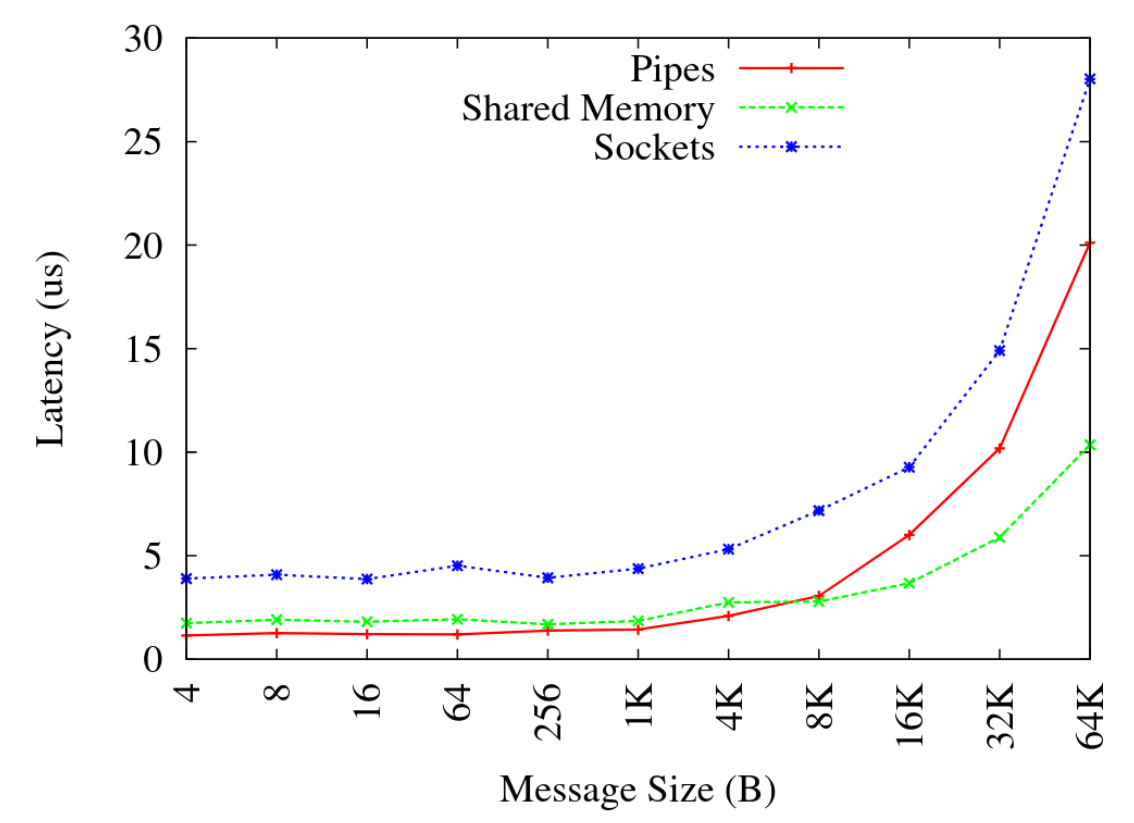
\includegraphics[width=10cm]{./Imagenes/venkataraman2015evaluation1.png}
    \caption{Ejemplo de uso de Tremor}%
    \label{fig:ipc_comparison1}
\end{figure}

\begin{figure}
    \centering
    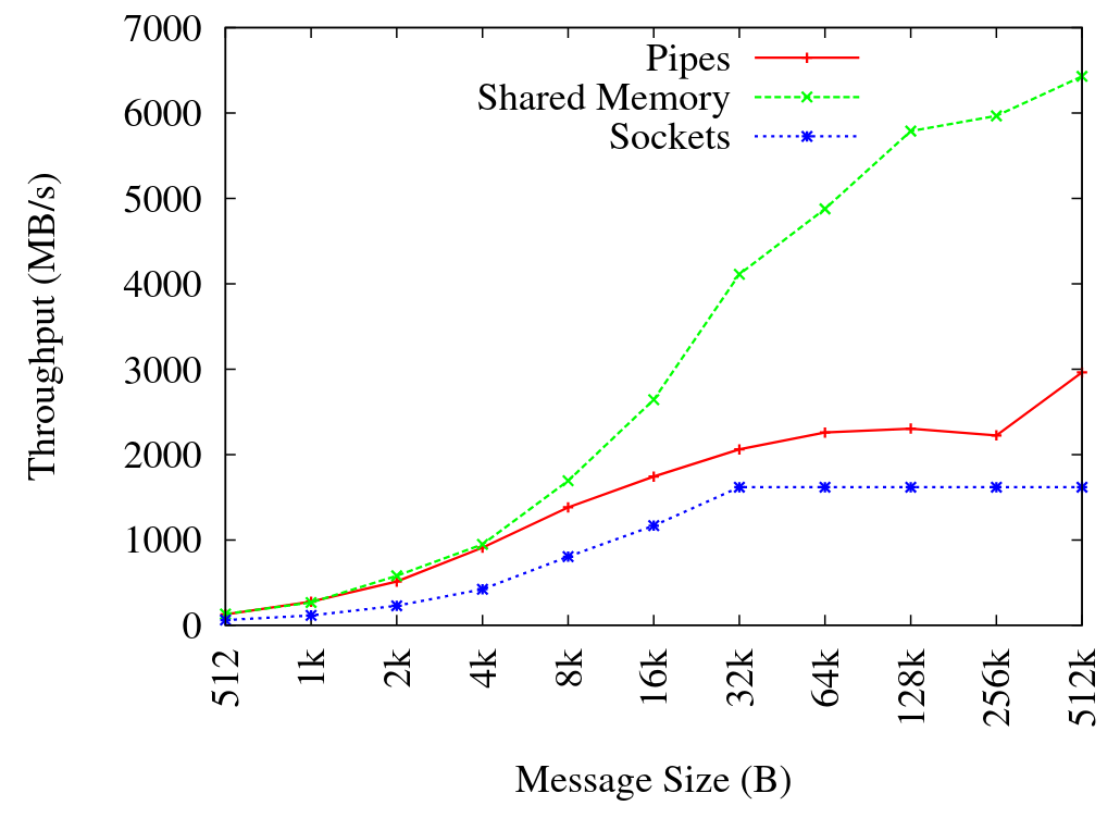
\includegraphics[width=10cm]{./Imagenes/venkataraman2015evaluation2.png}
    \caption{Ejemplo de uso de Tremor}%
    \label{fig:ipc_comparison2}
\end{figure}

\subsection{Cargado dinámico}

\subsection{WebAssembly}

\subsection{eBPF}

\section{Conclusión}

TODO: incluir eBPF

\begin{figure}
    \centering
    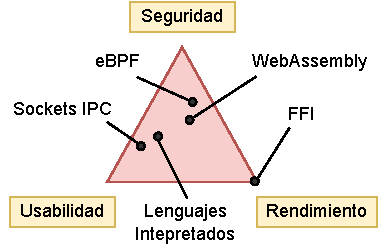
\includegraphics[width=10cm]{./Imagenes/triangle.pdf}
    \caption{Ejemplo de uso de Tremor}%
    \label{fig:tech_triangle}
\end{figure}
